\documentclass[10pt,twoside,a4paper]{book}
%\usepackage[options]{extension}
\usepackage{amssymb}
\usepackage{amsmath}
\usepackage{graphicx}
\usepackage[T1]{fontenc}
\usepackage{fancyhdr}
\pagestyle{fancy}
\usepackage[english,francais]{babel}

\graphicspath{ {./img/} }
%\setlength{\parindent}{0pt}
\author{Adela Patcas}
\title{Signal Spaces}

\lhead[\thepage]{1.10 Des exercices}
\rhead[Introduction et fondements]{\thepage}
\cfoot{}

\begin{document}

% PAGE 63
\setcounter{page}{63}

\begin{enumerate}
  \item[]
  \begin{enumerate}
    \item[] 
    \noindent
    Les quantités $A(j\omega)$ et $\phi (j\omega)$ correspondent à l'amplitude réciproque et au déphasage entre entrée et sortie.
    
    \item[(c)] Montrer que si les mesures d'amplitude/phase sont effectuées à $n$ fréquences différentes $\omega_1, \omega_2, \ldots, \omega_n$, alors les paramètres inconnus $a$ et $b$ peuvent être estimés en résolvant l'ensemble d'équations surdéterminé
    
    \begin{equation*}
      \begin{bmatrix}
        A(j\omega_1) & -\omega_1 \sqrt{1+1/tan^2 \phi (j\omega_1)} \\ 
        tan \phi (j\omega_1) & -\omega_1 \\
        A(j\omega_2) & -\omega_2 \sqrt{1+1/tan^2 \phi (j\omega_2)} \\
        tan \phi (j\omega_2) & -\omega_2 \\
        \vdots \\
        A(j\omega_1)  & -\omega_n \sqrt{1+1/tan^2 \phi (j\omega_n)} \\
        tan \phi (j\omega_n) & -\omega_n
      \end{bmatrix}
      \begin{bmatrix}
        b \\
        a
      \end{bmatrix}
      =
      \begin{bmatrix}
        0 \\
        \omega_1^2 tan \phi (j\omega_1) \\
        0 \\
        \omega_2^2 tan \phi (j\omega_2) \\
        \vdots \\
        0 \\
        \omega_n^2 tan \phi (j\omega_n)
      \end{bmatrix}.
    \end{equation*}
  \end{enumerate}

  \item[1.4-27] Vérifiez (1.38).
  \item[1.4-28] Montre que
  
  \begin{equation*}
    \sum_{t=-\infty}^{\infty} |y[t]|^2 = \frac{1}{2\pi} \int_{-\pi}^{\pi} G_{yy}(\omega)d\omega.
  \end{equation*}

  \noindent
  Astuce: rappelez-vous la transformée de Fourier inverse

  \begin{equation*}
    y[t] = \frac{1}{2\pi} \int_{-\pi}^{\pi} Y(\omega) e^{j\omega t} d\omega.
  \end{equation*}

  \item[1.4-29] Montrer que sous la condition que (1.39) soit vraie, la PSD satisfait
  
  \begin{equation*}
    S_{yy}(\omega) = \lim_{N \longrightarrow \infty} E \left[\frac{1}{N} \left| \sum_{n=1}^{N} y[n]e^{-j\omega n} \right|^2 \right].
  \end{equation*}

  \noindent
  Astuce: montrez et utilisez le fait que

  \begin{equation*}
    \sum_{n=1}^{N} \sum_{m=1}^{N} f(n-m) = \sum_{l=-N+1}^{N-1} (N-|l|) f(l).
  \end{equation*}

  \item[1.4-30] (Analyse modale) Les données suivantes sont mesurées à partir d'un système de troisième ordre:
  
  \begin{equation*}
    y = \{0.3200, 0.2500, 0.1000, -0.0222, 0.0006, -0.0012, 0.0005, -0.0001 \}.
  \end{equation*}

  \noindent
  Supposons que le premier indice de temps soit 0, de sorte que y[0] = 0,32.

  \begin{enumerate}
    \item Déterminez les modes du système et tracez-les dans le plan complexe.
    \item Les données peuvent être écrites sous la forme
    
    \begin{equation*}
      y[t] = c_1(p_1)^t + c_2(p_2)^t + c_3(p_3)^t \quad t \geq 0.
    \end{equation*}

    \noindent
    Déterminez les constantes $c_1$, $c_2$ et $c_3$.

    \item Pour explorer l'effet du bruit sur le système, ajoutez un bruit gaussien aléatoire à chaque point de données avec une variance a $\sigma^2 = 0.01$, puis trouvez les modes des données bruyantes. Répétez plusieurs fois (avec un bruit différent) et commentez la façon dont les estimations modales évoluent.
  \end{enumerate}

  \item[1.4-31] (Analyse modale) Si y[t] a deux sinusoïdes réelles,
  
  \begin{equation*}
    y[t] = A cos(\omega_1t + \theta_1) + B cos(\omega_2t + \theta_2),
  \end{equation*}

  \noindent
  et les fréquences sont connues, déterminer un moyen de calculer les amplitudes et les phases à partir de mesures aux instants $t_1, t_2, \ldots, t_N$.
\end{enumerate}

\par\noindent\rule{\textwidth}{0.6pt}

\begin{enumerate}
  \item[1.6-32] Montrer que $R^{-1}$ de (1.50) est correct.
  \item[1.6-33] Montrer que (1.51) découle de (1.47) et (1.50).
  
  % PAGE 64

  \item[1.6-34] Supposons que $X \sim \mathcal{N}(\mu_x, \sigma_X^2)$ et $N \sim \mathcal{N}(0, \sigma_n^2)$ soient des r.v.s gaussiennes distribuées indépendamment. Laisser
  
  \begin{equation*}
    Y = X + N.
  \end{equation*}

  \begin{enumerate}
    \item Déterminer les paramètres de la distribution de Y.
    \item Si $Y = y$ est mesuré, nous pouvons estimer $X$ en calculant la densité conditionnelle $f(X|y)$. Déterminez la moyenne et la variance de cette densité conditionnelle. Interpréter ces résultats en termes d'obtention d'informations sur $X$ si (i) $\sigma_n^2 \gg \sigma_x^2$ et (ii) $\sigma_n^2 \ll \sigma_x^2$.
  \end{enumerate}

  \item[1.6-35] Supposons que $X \sim \mathcal{N}(\mu_x, \sigma_X^2)$ et $Y \sim \mathcal{N}(\mu_y, \sigma_y^2)$ soient des r.v.s gaussiennes distribuées conjointement avec une corrélation $\rho$. Déterminez les paramètres de la distribution de $Z = aX + bY$.
  \item[1.6-36] Si $X \sim \mathcal{N}(0, 1)$, montrer que
  
  \begin{equation*}
    Y = \sigma X + \mu
  \end{equation*}

  \noindent
  est distribué comme $Y \sim \mathcal{N}(\mu, \sigma^2)$.

  \item[1.6-37] Soit $x_1, x_2, \ldots, x_n$ $n$ observations indépendantes d'une variable aléatoire gaussienne $X$ de moyenne et de variance inconnues. Nous souhaitons estimer la moyenne et la variance de $X$. 
  La densité conjointe de $n$ r.v.s gaussiennes indépendantes, conditionnée à la connaissance de la moyenne $\mu$ et de la variance $\sigma^2$, est

  \begin{equation*}
    f(x_1, x_2, \ldots, x_n | \mu , \sigma^2) = \frac{1}{(2 \pi )^{n/2} \sigma^n} exp \left[- \frac{1}{2\sigma^2} \sum_{i=1}^{n} (x_i - \mu)^2 \right].
  \end{equation*}

  \begin{enumerate}
    \item Déterminez une estimation du \textit{maximum de vraisemblance} de $\mu$ en maximisant cette densité conjointe par rapport à $\mu$ (c'est-à-dire, prenez la dérivée par rapport à $\mu$) . Appelons $\hat{\mu}$ l'estimation de la moyenne ainsi obtenue.
    \item Puisque $\hat{\mu}$ est une fonction de variables aléatoires, c'est lui-même une variable aléatoire. Déterminez la moyenne (valeur attendue) de $\hat{\mu}$. Une estimation dont la valeur attendue est égale à la valeur estimée est dite \textit{sans biais}.
    \item Déterminez la variance de $\hat{\mu}$.
    \item Déterminer une estimation pour $\sigma^2$.
  \end{enumerate}

  \noindent
  Il est naturel de se demander s'il existe un meilleur estimateur de la moyenne que celui "évident" qui vient d'être obtenu. Cependant, comme le montrera la section 12.3.2, cet estimateur est sans aucun doute le meilleur, dans le sens où il présente la variance la plus faible possible pour toute estimation non biaisée.
\end{enumerate}

\par\noindent\rule{\textwidth}{0.6pt}

\begin{enumerate}
  \item[1.7-38] Un processus aléatoire de Markov $X(t)$ a la propriété que
  
  \begin{equation*}
    P(X(t_3) = x_2|X(t_2) = x_2, X(t1) = x_1) = P(X(t_3) = x_3|X(t_2) = x_2)
  \end{equation*}

  \noindent
  quand $t_3>t_2>t_1$; c'est-à-dire que la probabilité dépend uniquement de l'événement conditionnant le plus récent. Nous abrégerons cela en utilisant la notation

  \begin{equation*}
    f(x_3|x_2, x_1) = f(x_3|x_2).
  \end{equation*}

  \begin{enumerate}
    \item Pour un processus de Markov, montrez que
    
    \begin{equation*}
      f(x_3, x_1|x_2) = f(x_3|x_2)f(x_2|x_1).
    \end{equation*}

    \noindent
    C'est la propriété d'indépendance conditionnelle ($x_3$ est indépendant de $x_1$, à condition que ils sont conditionnés chacun à une observation intermédiaire $x_2$).
    
    \item Supposons maintenant que $X(t)$ soit un processus aléatoire gaussien, et supposons (pour des raisons de commodité uniquement) qu'il soit de moyenne nulle. Laisser
    
    \begin{equation*}
      r_x(t,s) = E[X(t)X(s)].
    \end{equation*}

    \noindent
    Si $X(t)$ est aussi Markov, montrer que

    \begin{equation*}
      r_x(t_3,t_1) = \frac{r_x(t_3,t_2)r_x(t_2,t_1)}{r_x(t_2,t_2)}.
    \end{equation*}

    \noindent
    Astuce: utilisez le fait que $E[E[X(t_3)X(t_1)|X(t_2)]] = E[X(t_3)X(t_1)]$ et utilisez la formule pour l'espérance conditionnelle dérivée de (1.52).
  \end{enumerate}

  % PAGE 65
  \item[1.7-39] Pour la matrice de probabilité de transition d'état A donnée en (1.58), trouvez un vecteur de probabilité \textbf{p} tel que
  
  \begin{equation*}
    Ap=p
  \end{equation*}

  \noindent
  Un tel vecteur de probabilité est appelé probabilité \textit{en régime permanent} du modèle de Markov.
\end{enumerate}

\par\noindent\rule{\textwidth}{0.6pt}

\begin{enumerate}
  \item[1.8-40] Montrez que $\sqrt{3}$ est irrationnel.
  \item[1.8-41] Montrer qu'il existe un nombre infini de nombres premiers. Astuce: utilisez une preuve par contradiction, en supposant qu'il n'existe qu'un nombre fini de nombres premiers. 
  Construisez ensuite un numéro $2 \cdot 3 \cdot 5 \cdot \cdots \cdot p + 1$, où $p$ est le dernier nombre premier supposé, et montrer que celui-ci n'est divisible par aucun des nombres premiers répertoriés.
  \item[1.8-42] Montrer que si $m^2$ est pair, alors $m$ doit être pair.
  \item[1.8-43] Par essais et erreurs, déterminez une formule plausible pour
  
  \begin{equation*}
    \sum_{i=0}^{n}2^i.  
  \end{equation*}

  \noindent
  Prouvez ensuite par récurrence que votre formule est correcte.
  \item[1.8-44] Déterminer (par expérience) une formule plausible pour la somme des $n$ premiers entiers impairs
  
  \begin{equation*}
    1+3+5+ \cdots + (2n-1).
  \end{equation*}

  \noindent
  Prouvez ensuite par récurrence que votre formule est correcte.
  \item[1.8-45] Déterminer (par expérience) une formule plausible pour
  
  \begin{equation*}
    \sum_{i=1}^{n} \frac{1}{i^2+i}.
  \end{equation*}

  \noindent
  Prouvez ensuite par récurrence que votre formule est correcte.
  \item[1.8-46] Montrer par récurrence, pour tout entier positif $n$, que $n^3-n$ est divisible par 3.
  \item[1.8-47] The quantity

  \begin{equation*}
    \begin{pmatrix}
      n \\
      k 
    \end{pmatrix} = \frac{n!}{k!(n-k)!}
  \end{equation*}

  \noindent
  est le nombre de façons de choisir $k$ objets parmi $n$ objets, où $n \geq k$. La quantité (;) est également connue sous le nom de \textit{coefficient binomial}. Nous lisons la notation (:) comme "$n$ choisit $k$".
  
  \noindent
  Montrer par induction que, pour $1 \leq k \leq n$,

  \begin{equation}
    \begin{pmatrix}
      n+1 \\
      k 
    \end{pmatrix} =
    \begin{pmatrix}
      n \\
      k 
    \end{pmatrix} +
    \begin{pmatrix}
      n \\
      k-1 
    \end{pmatrix}
  \end{equation}
  \item[1.8-48] Montrer par récurrence que, pour $n \geq 0$,
  
  \begin{equation*}
    \sum_{i=0}^{n} \begin{pmatrix}
      n \\
      k 
    \end{pmatrix} =2^n.
  \end{equation*}
  \item[1.8-49] Montrer par induction que
  
  \begin{equation}
    (x+y)^n = \sum_{k=0}^{n} \begin{pmatrix}
      n \\
      k 
    \end{pmatrix} x^k y^{n-k}
  \end{equation}

  \noindent
  Cette formule importante est connue sous le nom de \textit{théorème binomial}.

  % PAGE 66

  \item[1.8-50] Prouver ce qui suit par induction:
  
  \begin{equation*}
    \sum_{k=1}^{n}k^2 = \frac{n(n+1)(2n+1)}{6}.
  \end{equation*}
  \item[1.8-51] Prouver ce qui suit par induction:
  
  \begin{equation*}
    \sum_{k=1}^{n}r^k = \frac{r^{n+1}-1}{r-1} \quad r \neq 1
  \end{equation*}
  \item[1.8-52] Prouver par induction que
  
  \begin{equation*}
    \frac{1}{\sqrt{4n+1}} < \frac{1}{2} \cdot \frac{3}{4} \cdot \cdots \cdot \frac{2n-3}{2n-2} \cdot \frac{2n-1}{2n} < \frac{1}{\sqrt{3n+1}}
  \end{equation*}

  \noindent
  pour les entiers $n \geq 1$.
  \item[1.8-53] Montrer par récurrence que, pour $x,y \in \mathbb{Z}$ et tout entier non négatif $n$, $(x-y)$ divise $x^n-y^n$. Ceci s'écrit
  
  \begin{equation*}
    (x-y)|(x^n-y^n).
  \end{equation*}
\end{enumerate}

\par\noindent\rule{\textwidth}{0.6pt}

\begin{enumerate}
  \item[1.9-54] Préparez un tableau montrant le contenu de stockage et les sorties pour le LFSR indiqué dans l'illustration ci-jointe, avec les conditions initiales indiquées dans les éléments de retard. Déterminez également le polynôme de connexion $C(D)$.
  %\begin{figure}[h]
  %  \centering
  %  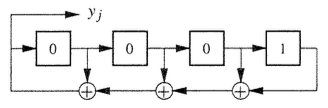
\includegraphics[scale=0.8]{fig1.1}
  %\end{figure}

  \item[1.9-55] Considérons le LFSR décrit par le polynôme
  
  \begin{equation*}
    C(D) = 1 + D + D^2 + D^3.
  \end{equation*}

  \begin{enumerate}
    \item Dessinez le schéma fonctionnel LFSR en utilisant à la fois la réalisation montrée dans la figure 1.20 et la réalisation montrée dans 1.21.
    \item Pour la condition initiale $\{0, 0, 1\}$, tracez le fonctionnement des deux réalisations du LFSR et vérifiez que la séquence de sortie de chacune est la même. Combien y a-t-il d'états de district?
  \end{enumerate}

  \item[1.9-56] Considérons le LFSR décrit par le polynôme
  
  \begin{equation*}
    1 + D^2 + D^3.
  \end{equation*}

  \begin{enumerate}
    \item Dessinez le schéma fonctionnel LFSR en utilisant à la fois la réalisation montrée dans la figure 1.20 et la réalisation montrée dans 1.21.
    \item Pour la condition initiale $\{0, 0, 1\}$, tracez le fonctionnement des deux réalisations du LFSR et vérifiez que la séquence de sortie de chacune est la même. Combien y a-t-il d'états de district?
  \end{enumerate}

  \item[1.9-57] Étant donné la séquence $\{0, 0, 0, 1, 0, 1, 0\}$,
  
  \begin{enumerate}
    \item Déterminez le LFSR le plus court qui pourrait produire cette séquence, en effectuant les calculs à la main.
    \item Vérifiez votre travail en utilisant l'Algorithme 1.2 dans \textsc{Matlab}.
  \end{enumerate}

  \item[1.9-58] Montrez que pour $j=0,1,\ldots,n$, la sortie du LFSR avec le polynôme de connexion $C^{[n+1]}(D)$ comme dans (1.65) avec $A=-d_m^{-1}d_n$ et $l=n-m$ satisfait $d_j = 0$ (pas de divergence).
  
  % PAGE 67

  \item[1.9-59] Écrivez la séquence de sortie sous forme de polynôme
  
  \begin{equation*}
    Y(D)=y_0+y_1D+y_2 D^2 + \cdots .
  \end{equation*}

  \begin{enumerate}
    \item En utilisant (1 63), montrez que le coefficient j dans Y(D)C(D) disparaît pour J = p p +1 où deg(C(D)) = p. On peut donc écrire
    
    \begin{equation*}
      C(D)Y(D)=Z(D).
    \end{equation*}

    où

    \begin{equation*}
      Z(D)=z_0+z_1D+ \cdots +z_{p-1}D^{p-1}.
    \end{equation*}

    \noindent
    Ainsi, connaissant $Z(D)$, nous pouvons trouver le résultat par division polynomiale longue:

    \begin{equation}
      Y(D)= \frac{Z(D)}{C(D)}.
    \end{equation}

    \item Montrer que les coefficients de $Z(D)$ peuvent être liés aux conditions initiales du LFSR par
    
    \begin{equation*}
      \begin{bmatrix}
        1 & 0 & \cdots & & 0 \\
        c_1 & 1 & \cdots & & 0 \\
        c_2 & c_1 & \cdots & & 0 \\
        \vdots \\
        c_{p-1} & c_{p-2} & \cdots & c_1 & 1
      \end{bmatrix}
      \begin{bmatrix}
        y_0 \\
        y_1 \\
        y_2 \\
        \vdots \\
        y_{p-1}
      \end{bmatrix}=
      \begin{bmatrix}
        z_0 \\
        z_1 \\
        z_2 \\
        \vdots \\
        z_{p-1}
      \end{bmatrix}.
    \end{equation*}
  \end{enumerate}
  \item[1.9-60] Soit $C(D) = 1+D^2+D^3$, de contenu initial $\{y_0,y_1,y_2\}=\{1,0,0\}$. Déterminez les six premières sorties en utilisant la division polynomiale longue (1.84). Comparez les résultats à ceux obtenus directement du LFSR.
  \item[1.9-61] Déterminez la séquence $\{y_i\}$ de longueur sept générée par $C(D)=1+D+D^3$, et appelez sa longueur $N$. Calculez ensuite la fonction d'autocorrélation cyclique
  
  \begin{equation*}
    \rho(k)=\frac{1}{N} \sum_{i=0}^{N-1} y_i y_{((i-k))},
  \end{equation*}

  \noindent
  où $y_i y_{((i-k))}$ signifie que l'indice est calculé modulo $N$. Tracez cette fonction d'autocorrélation.
\end{enumerate}

\section{Les références}

\lhead[\thepage]{1.11 Les références}
\noindent
La théorie des systèmes linéaires présentée ici à grands traits est décrite de manière beaucoup plus détaillée dans [284] et [164]. 
Notre brève introduction à la prédiction linéaire est présentée de manière plus détaillée dans [68,132], tandis que beaucoup plus d'informations sur l'analyse spectrale apparaissent dans [174,220]. 
Les applications du filtrage adaptatif mises en évidence ici sont discutées en profondeur dans [132] et [368]. Le modèle de Markov caché est présenté en 1266, 681 et 12651. 
Pour une introduction agréable et lisible aux preuves, avec une variété de suggestions et d'exemples et une bonne base mathématique, [352] est recommandé. Un livre qui suscite la réflexion sur la pensée mathématique est [256].

L'algorithme de Massey est présenté dans [221]. Une excellente présentation de l'algorithme se trouve dans [32]. Le livre [I091 fournit une introduction aux LFSR et l'article [288] une discussion intéressante sur les séquences de longueur maximale décimées. 
Les applications des LFSR aux communications à spectre étalé sont discutées dans [387].

\newpage
\thispagestyle{empty}
\newpage

% PAGE 71
\setcounter{chapter}{1}
\chapter{Espaces de signalisation}

\thispagestyle{empty}

\renewenvironment{quote}{%
  \list{}{%
    \leftmargin0.5cm   % this is the adjusting screw
    \rightmargin\leftmargin
  }
  \item\relax
}
{\endlist}

\begin{quote}
  Le langage constitue un puissant filet lâche avec lequel aller à la pêche aux faits simples, alors que les faits sont infinis.
  \begin{flushright}
  {--\textit{Edward Abbey} \\ Desert Solitaire}
  \end{flushright}
\end{quote}
\begin{quote}
  Les débutants ne sont pas préparés à une véritable rigueur mathématique; ils n'y verraient que des subtilités creuses et ennuyeuses. Ce serait une perte de temps que de vouloir les rendre plus exigeants; il leur faut parcourir rapidement et sans s'arrêter le chemin qui a été parcouru lentement par les fondateurs de la science.
  \begin{flushright}
  {--\textit{Henri Poincare} \\ Science and Hypothesis}
  \end{flushright}
\end{quote}
\vspace{7mm}

\noindent
Ce chapitre concerne principalement deux types d'objets mathématiques: les espaces métriques et les espaces vectoriels linéaires. L'idée derrière un espace métrique est 
simplement que nous fournissons un moyen de mesurer la distance entre des objets mathématiques, tels que des ensembles, des points, des fonctions ou des séquences. 
Avec cette notion de distance nous pourrons généraliser certains des concepts familiers du calcul, comme la continuité ou la convergence, au-delà des opérations sur une 
seule dimension vers les opérations dans des dimensions supérieures.

Le concept d'espace vectoriel est également simple: il s'agit d'un ensemble d'objets qui peuvent être combinés entre eux à l'aide de combinaisons linéaires. 
Mais la théorie des espaces vectoriels a des ramifications considérables, couvrant une partie importante de la théorie du traitement du signal. Un élément clé de la 
théorie de l'espace vectoriel est que, dans un sens géométriquement utile, les \textbf{fonctions (c'est-à-dire les signaux) peuvent être considérées comme des vecteurs}. 
Cette compréhension géométrique fournit un outil puissant pour l'analyse du signal. Dans ce chapitre, la théorie de base et la notation des espaces vectoriels sont développées. 
Dans le chapitre 3, nous mettons cette notion en pratique dans diverses applications, notamment le filtrage optimal (moindres carrés et carrés moyens minimaux), les transformations, 
la compression de données, l'échantillonnage et l'interpolation.

\lhead[\thepage]{2.1 Espaces métriques}
\rhead[Espaces de signalisation]{\thepage}

Dans notre étude des espaces métriques et des espaces vectoriels, l'intention est de fournir un cadre pour la discussion générale des signaux. Avant de commencer ce chapitre, 
le lecteur est encouragé à revoir les définitions de base des fonctions et des ensembles apparaissant dans l'annexe A. Dans cette étude, la notation matricielle est largement 
utilisée dans les sections, donc la révision des notations matricielles de base présentées dans l'annexe C est également recommandée.

Dans le développement de ce chapitre, nous construisons successivement des \textbf{espaces métriques}, des \textbf{espaces vectoriels}, des \textbf{espaces vectoriels normés}, puis des espaces de \textbf{produits internes normés}. 
Cela nous amènera à l'idée importante des projections et des projections orthogonales. La projection orthogonale sera un outil d'une importance capitale pour nous dans le prochain chapitre, 
où elle sera utilisée comme base géométrique pour le filtrage et la prédiction par les moindres carrés et les carrés moyens minimaux.

% PAGE 72

\section{Espaces métriques}

\noindent
Nous pouvons considérer que les signaux (fonctions) qui nous intéressent dans un problème particulier sont membres d'un ensemble $X$. En étudiant et en appliquant ces signaux, nous pouvons être intéressés à comprendre 
comment un signal se compare aux autres signaux de cet ensemble. Une façon d'y parvenir consiste à mesurer une "distance" entre les signaux en utilisant une mesure de distance qui est à la fois mathématiquement significative 
et physiquement significative. Les aspects mathématiques d'une fonction de mesure utile sont exprimés dans la définition suivante.
\vspace{4mm}

\noindent
\textbf{Définition 2.1} Une \textbf{métrique} $d: X \times X \longrightarrow \mathbb{R}$ est une fonction utilisée pour mesurer la distance entre les éléments d'un ensemble $X$. 
Pour être une métrique, elle doit satisfaire aux propriétés suivantes. pour $x, y \in \textit{X}$:
\vspace{2mm}

M1 $d(x, y) = d(y, x)$.

M2 $d(x, y) \geq 0$.

M3 $d(x, y) = 0$ si et seulement si $x = y$.

M4 Pour tous les points $x, y, z \in \textit{X}$,

\begin{equation}
       d(x, z) \leq d(x, y) + d(y, z).
\end{equation}

\vspace{4mm}

\noindent
\textbf{Exemple 2.1.1} Pour $x, y \in \mathbb{R}$ nous pouvons définir une métrique en utilisant la fonction valeur absolue par

\begin{equation*}
       d(x, y) = |x - y|.
\end{equation*}

\noindent
Les propriétés requises d'une métrique sont toutes satisfaites. La dernière propriété découle de \textbf{l'inégalité triangulaire}, 
ainsi appelé en raison de la relation qui s'impose sur les glissières d'un triangle plan. Soit $x$,$y$ et $z$ désignent les coins d'un triangle, 
comme le montre la figure 2.1. Alors $d(x, z)$ est la longueur d'un côté,

%\begin{figure}[h]
%  \centering
%  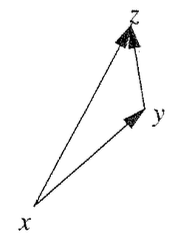
\includegraphics[scale=0.8]{fig2.1}
%  \caption{Illustration de l'inégalité triangulaire}
%\end{figure}

\noindent
$d(y, z)$ est la longueur du deuxième côté et $d(x, z)$ est la longueur du troisième côté. 
La longueur du le troisième côté ne peut pas être plus long que la longueur des deux premiers côtés.

\vspace{4mm}

Il existe une variété de mesures utilisées; l'exemple suivant en illustre quelques-uns.

% PAGE 73
\vspace{4mm}
\noindent
\textbf{Exemple 2.1.2} Soit $X$ l'ensemble des nombres dans $\mathbb{R}^n$. Soit $x \in \mathbb{R}^n$ et $y \in \mathbb{R}^n$.

\begin{enumerate}
  \item La métrique $d_1:\mathbb{R}^n \times \mathbb{R}^n \longrightarrow \mathbb{R}$ définie par
  
  \begin{equation*}
    d_1(x, y) = \sum_{i=1}^{n} |x_i - y_i|
  \end{equation*}
  
  \noindent
  est appelée métrique $l_1$, également connue sous le nom de métrique de Manhattan, car la distance mesurée dans une ville disposée sur une grille 
  cartésienne doit suivre tout droit le long des rues. La satisfaction de la propriété (2.1) pour cette métrique découle de l'inégalité troangle appliquée à chaque terme.
  \item La métrique $d_2:\mathbb{R}^n \times \mathbb{R}^n \longrightarrow \mathbb{R}$ définie par
  
  \begin{equation*}
    d_2(x, y) = \left({\sum_{i=1}^{n} |x_i - y_i|^2}\right)^{1/2}
  \end{equation*}

  \noindent
  est appelée métrique $l_2$. Il représente la distance euclidienne entre les points. Le fait que cette métrique satisfait la propriété (2.1) est prouvé dans la section 2.6.
  \item En généralisant les deux premières métriques, nous avons
  
  \begin{equation*}
    d_p(x, y) = \left({\sum_{i=1}^{n} |x_i - y_i|^p}\right)^{1/p}
  \end{equation*}

  \noindent
  C'est la métrique $l_p$. Le fait que cette métrique satisfasse (2.1) découle de l'inégalité de Minkowski, qui est démontrée dans l'annexe A.
  \item Comme $p \longrightarrow \infty$, la métrique $l_p$ devient la métrique $l_\infty$,
  
  \begin{equation*}
    d_\infty(x, y) = \max\limits_{i=1,2,...,n} |x_i - y_i|.
  \end{equation*}
\end{enumerate}

\vspace{4mm}
\noindent
\textbf{Exemple 2.1.3} Considérons un vecteur $x \in \mathbb{R}^n$ qui doit être approché (quantifié) par un vecteur comme $\hat{x}$ illustré sur la figure 2.2. 
Pour avoir une bonne représentation des données, nous souhaitons que $\hat{x}$ "ressemble" à x, selon certains critères, et le quantificateur doit être conçu en gardant cela à l'esprit. 
Bien que de nombreuses métriques différentes aient été examinées, les métriques utilisées dans la conception du quantificateur s'avèrent souvent être l'une de celles mentionnées 
ci-dessus, telles que $d_1(x, \hat{x})$ ou $d_2(x, \hat{x})$.

%\begin{figure}[h]
%  \centering
%  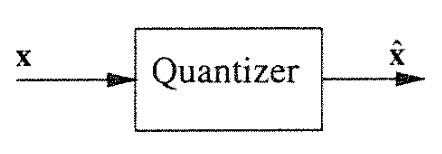
\includegraphics[scale=0.8]{fig2.2}
%  \caption{Quantification du vecteur x}
%\end{figure}

\vspace{4mm}
\noindent
\textbf{Exemple 2.1.4} Soit \textbf{x} une séquence binaire, $\textbf{x} = \{x_0, x_1,...,x_{n-1}\}$, où $x_i$ vaut 0 ou 1. Cette séquence est transmise via un canal où elle peut être 
corrompue par du bruit. La séquence reçue est $\textbf{y} = \{y_0, y_1,...,y_{n-1}\}$. Lors de la réception de telles séquences, l'objectif d'une bonne réception est que les bits de \textbf{y}
correspondent aux bits de \textbf{x}. Une métrique appropriée pour ce critère est la \textit{distance de Hamming} entre les séquences, qui est le nombre de places où $x_i$ et $y_i$ sont différents,

\begin{equation*}
  d_H(x, y) = \sum_{i=0}^{n-1} h(x_i - y_i)
\end{equation*}

\noindent
où

\begin{equation*}
  h(x, y) = \begin{cases} 1 & si \ x - y \neq 0 \\
    0 & si \ x - y = 0.
        \end{cases}
\end{equation*}

\noindent
Lorsque \textbf{x} et \textbf{y} sont des séquences binaires, alors la distance de Hamming qui les sépare peut s'écrire

\begin{equation*}
  d_H(x, y) = \sum_{i=0}^{n-1} x_i \oplus y_i ,
\end{equation*}

\noindent
dans lequel $\oplus$ désigne l'addition modulo 2.

% PAGE 74

\vspace{4mm}
\noindent
\textbf{Définition 2.2} Un \textbf{espace métrique} $(X, d)$ est un ensemble $X$ avec une métrique $d$.

\noindent
Il existe de nombreux espaces métriques possibles. Nous commençons par les espaces métriques définis pour les séquences.

\vspace{4mm}
\noindent
\textbf{Exemple 2.1.5}
\begin{enumerate}
  \item L'ensemble $\mathbb{R}^n$ équipé de la métrique $d_2(x, y)$ est un espace métrique.
  \item Soit $l_p = l_p(0, \infty)$ l'ensemble constitué de toutes les séquences infinies de nombres réels ou complexes $\{x_0, x_1,...,x_{n-1}\}$ tels que
  $\sum_{i=0}^{\infty} |x_i|^p < \infty$. Nous prendrons $1 \leq p < \infty$. La fonction
  \begin{equation*}
    d_p(x, y) = \left[{\sum_{i=0}^{\infty} |x_i - y_i|^p}\right]^{1/p}
  \end{equation*}
  \noindent
  définit une métrique sur $l_p$, que nous appellerons la métrique $l_p$. Nous appelons cet espace métrique l'espace $l_p(0, \infty)$, ou simplement l'espace $l_p$. 
  Il s'agit d'un espace de dimension infinie appelé \textit{espace de séquence}.

  L'ensemble des séquences bilatérales $\{...,x_{-1}, x_0, x_1,...\}$ de métrique $d_p$ donne l'espace métrique $l_p(-\infty, \infty)$.

  Dans les applications de traitement du signal en temps discret, nous traitons le plus souvent de l'espace $l_1$ ou de l'espace $l_2$, le premier parce que les valeurs absolues sont faciles à calculer, et le second parce que la fonction métrique quadratique est facilement différentiable.s
  \item L'espace $l_\infty(0, \infty)$ est constitué de toutes les suites de nombres $\{x_0, x_1, x_2,...\}$ telles que $|x_n| \leq M$ pour une borne finie $M$ , équipée de la métrique
  
  \begin{equation}
    d_\infty(x, y) = \sup\limits_n |x_n - y_n| .
  \end{equation}
  \noindent
  Voir encadré 2.1. L'espace correspondant des séquences bilatérales est noté $l_\infty(-\infty, \infty)$.
\end{enumerate}

\vspace{4mm}
Il existe également de nombreux espaces métriques utiles définis sur les fonctions. Ces espaces de dimension infinie sont appelés \textit{espaces fonctionnels}.

\vspace{4mm}
\noindent
\textbf{\textit{L'espace métrique} $(C[a, b], d_p)$.} Soit $X = C[a, b]$ l'ensemble des fonctions continues à valeurs réelles (ou à valeurs complexes) définies sur l'intervalle $[a, b]$, avec $b > a$. Nous pouvons définir une

% Box 2.1 Sup and inf
\vspace{7mm}

\fbox{%
    \parbox{\textwidth}{%
\textbf{Encadré 2.1: Sup et inf}
\par\noindent\rule{\textwidth}{1pt}
Pour un ensemble $S \subset \mathbb{R}$, la moindre limite supérieure (LUB) est le plus petit nombre $z$ tel que $z \geq x$ pour chaque $x \in S$. Le LUB d'un ensemble $S$ est appelé le \textbf{sup} (supremum) de l'ensemble. S'il n'y a pas de nombre supérieur à tous les éléments de $S$, 
alors $sup(S) = \infty$. De même, la plus grande limite inférieure (GLB) d'un ensemble est le plus grand nombre $w$ tel que $w \leq x$ pour chaque $x \in S$. Le GLB est appelé l'\textbf{inf} (infimum) de $S$. S'il n'y a pas de nombre inférieur à tous les éléments de $S$, alors $inf(S) = -\infty$.

L'inf et le sup sont respectivement des généralisations de min et max. Généralement, inf et sup sont utilisés lorsqu'il existe un continuum de valeurs sur lequel trouver le max ou le min, ou lorsque les extrema peuvent être infinis.

\textbf{Exemple 2.1.6} Soit $S = (2, 5) \subset \mathbb{R}$. (Il s'agit d'un ensemble ouvert et ne contient pas les points de terminaison.) Ensuite,
\begin{equation*}
  sup(S) = 5,  inf(S) = 2.
\end{equation*}

Soit $T = [4, 7)$. Alors $inf(T) = 4$ et $sup(T) = 7$. Soit $U = (1, \infty)$. Alors $inf(U) = 1$ et $sup(U) = \infty$
}%
}
\vspace{7mm}

% PAGE 75
\noindent
métrique sur les fonctions $x$ et $y$ dans $X$ par

\begin{equation}
  d_p(x, y) = \left[{\int_{a}^{b} |x(t) - y(t)|^p dt}\right]^{1/p} ,
\end{equation}

\noindent
où $1 \leq p < \infty$. Cela donne l'espace métrique $(C[a, b], d_p)$. La métrique $d_p$ entre les fonctions est appelée métrique $L_p$. Il faut établir que (2.3) est, en fait, une métrique. Pour $p = 2$, cela est établi à l'aide de l'inégalité de Cauchy-Schwarz (voir section 2.6). 
Pour les autres valeurs de $p$, l'inégalité de Minkowski démontrée en annexe A est utilisée.

\vspace{4mm}
\noindent
\textbf{\textit{L'espace métrique} $(C[a, b], d_\infty)$.} En laissant $p \longrightarrow \infty$ dans la définition de la dernière métrique, on obtient (voir encadré 2.1),

\begin{equation}
  d_\infty(x, y) = sup\{|x(t) - y(t)| : a \leq t \leq b\} ,
\end{equation}

\noindent
Autrement dit, la distance entre les fonctions est obtenue au point où les fonctions sont les plus éloignées. Cet espace métrique est noté $(C[a, b], d_\infty)$ ou, plus simplement, $C[a, b]$ (la métrique étant entendue par convention).

La différence entre les espaces métriques $(C[a, b], d_\infty)$ et $(C[a, b], d_p)$ peut être appréciée en considérant les fonctions illustrées dans la figure 2.3. Soit $X = C[0, T]$, et soit $x_0$ un point de $X$ (une fonction). 
La figure 2.3(a) montre la région dans laquelle toutes les fonctions $x$ qui satisfont

\begin{equation*}
  d_\infty(x_0, x) < \epsilon
\end{equation*}

%\begin{figure}[h]
%  \centering
%  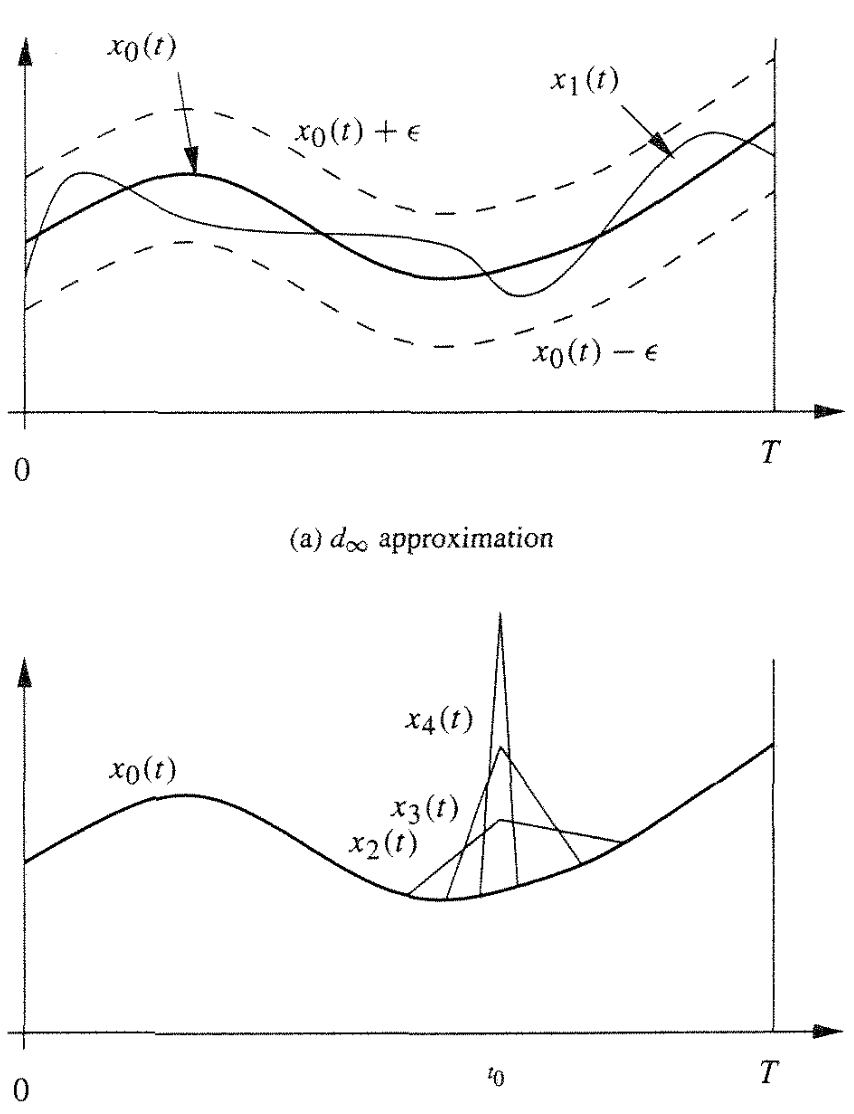
\includegraphics[scale=0.8]{fig2.3}
%  \caption{Comparaison des métriques $d_1$ et $d_2$}
%\end{figure}

% PAGE 76
\noindent
doit tomber. Par exemple, la fonction $x_1(t)$, comme indiqué, se situe dans la région. Même s'il peut y avoir des agitations dans la région, la fonction n'est jamais autorisée à s'échapper.

En revanche, la figure 2.3(b) illustre certaines fonctions qui satisfont

\begin{equation*}
  d_2(x_0, x) < \epsilon.
\end{equation*}

\noindent
Autrement dit, ce sont des fonctions pour lesquelles

\begin{equation*}
  \int_{0}^{T} (x_0(t) - x(t))^2 dt < \epsilon.
\end{equation*}

\noindent
À tout moment $t_0$ donné, il peut y avoir un écart significatif par rapport à $x_0(t)$ , tant que la région sur laquelle l'écart se produit n'est pas trop longue. Plus la zone de déviation est étroite, plus la déviation peut être importante. 
Si $x(t)$ est une approximation de $x_0(t)$, l'utilisation de la métrique $d_\infty$ pour exprimer le critère d'approximation fournit une limite supérieure à l'erreur d'approximation $x(t) - x_0(t)$ qui ne peut pas être obtenue en utilisant la métrique $d_p$ pour $1 \leq p < \infty$.

\vspace{4mm}
\noindent
\textbf{\textit{L'espace métrique} $L_p[a, b]$.} Soit $L_p[a, b]$ l'ensemble des fonctions $x(t)$ à valeurs réelles ou complexes définies sur l'intervalle $t \in [a, b]$ telles que

\begin{equation*}
  \int_{a}^{b} |x(t)|^p dt < \infty,
\end{equation*}

\noindent
où $1 \leq p < \infty$. Cet ensemble, équipé de la métrique $d_p$ de (2.3), forme l'espace métrique $(L_p[a, b], d_p)$ ou, plus simplement, $L_p[a, b]$. Lorsque l'intervalle est compris, il est souvent écrit simplement par $L_p$. La métrique (2.3) est souvent appelée métrique $L_p$.

Plusieurs aspects techniques associés à l'espace L sont abordés dans la section 2.1.3. Pour de nombreux problèmes d'intérêt technique, ces détails techniques ne présentent pas de difficulté, mais ils méritent une certaine attention.

\vspace{4mm}
\noindent
\textbf{\textit{L'espace métrique} $L_\infty[a, b]$.} Soit $L_\infty[a, b]$ l'ensemble des fonctions $x(t)$ à valeurs réelles ou complexes définies sur l'intervalle $[a, b]$ telles que

\begin{equation*}
  \sup_{t \in [a, b]} |x(t)| < \infty.
\end{equation*}

\noindent
Cet ensemble, muni de la métrique $d_\infty$ de (2.4), est un espace métrique.

\subsection{Quelques termes topologiques}
\noindent
Une fois la notion de métrique établie, nous pouvons introduire quelques concepts élémentaires de la topologie par ensembles de points.

Dans un espace métrique $X$, la \textbf{boule} ou \textbf{sphère} centrée en $x_0$ de rayon $\delta$ est l'ensemble des points qui sont à une distance $\delta$ de $x_0$:

\begin{equation}
  B(x_0, \delta) = \{x \in X : d(x_0, x) < \delta\}.
\end{equation}

\noindent
Une telle boule est aussi dite un \textbf{voisinage} de $x_0$: c'est l'ensemble des points qui habitent à proximité de $x_0$.

\vspace{4mm}
\noindent
\textbf{Définition 2.3} Un point $x_0 \in X$ est \textbf{intérieur} à un ensemble $S \subset X$ si tous les points suffisamment proches de $x_0$ sont dans $S$. Autrement dit, il existe $\delta > 0$ tel que $B(x_0, \delta) \subset S$.

\textbf{L'intérieur} d'un ensemble $S$ est l'ensemble de tous les points de $x$ qui sont intérieurs à l'ensemble. Un point $x_0  \notin S$ est \textbf{extérieur} s'il existe un voisinage de $x_0$ qui est à l'extérieur (ne coupe pas) $S$.

\vspace{2mm}
La figure 2.4 illustre un point intérieur, un point extérieur et un point qui n'est ni intérieur ni extérieur.

% PAGE 77

%\begin{figure}[h]
%  \centering
%  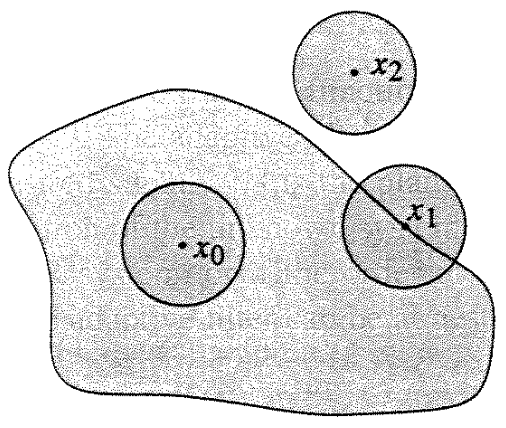
\includegraphics[scale=0.8]{fig2.4}
%  \caption{$x_0$ est intérieur, $x_2$ est extérieur et $x_2$ n'est ni intérieur ni extérieur}
%\end{figure}

\vspace{4mm}
\noindent
\textbf{Définition 2.4} Un ensemble $S$ est \textbf{ouvert} si tout point de $S$ est intérieur.

\vspace{4mm}
\noindent
\textbf{Exemple 2.1.7} L'ensemble $S = (0, 1) \subset \mathbb{R}$ est un ensemble ouvert. Nous montrerons que tout point est intérieur. Soit $x_0 \in S$. Alors la voisinage $B(x_0, \delta)$, où

\begin{equation*}
  \delta = \frac{1}{2} min(x_0, 1 - x_0),
\end{equation*}

\noindent
est un sous-ensemble de $S$ pour tout $x_0 \in S$.

L'ensemble $Y = [0, 1] \subset \mathbb{R}$ (y compris les points finaux) n'est pas ouvert. Le point 0 n'est entouré d'aucun quartier entièrement situé en $Y$.

Il est simple de montrer que les unions finies et les intersections d'ensembles ouverts sont ouvertes.

\vspace{4mm}
\noindent
\textbf{Définition 2.5} Un ensemble $S \subset X$ est dit \textbf{fermé} si le complémentaire de $S$ est un ensemble ouvert.

\vspace{4mm}
\noindent
\textbf{Exemple 2.1.8} Soit $X = (0, 4)$ et soit $S = [1, 2] \subset X$. Alors $\bar{S} = (0,1) \cup (2, 4)$. C'est l'union de deux ensembles ouverts, et donc ouvert. Donc $S$ doit être fermé.

\vspace{2mm}
Dans de nombreux cas dans ce livre, nous utiliserons des ensembles ouverts car ils ne peuvent pas contenir un seul point. Par exemple, dans certains résultats sur l'optimisation, nous pourrions énoncer quelque chose comme: "$f(t)$ est continu dans un voisinage ouvert autour de $t_0$." 
Cela signifie que nous pouvons examiner les points autour de $t_0$ - dans au moins certains quartier - et y utiliser la continuité.

\vspace{4mm}
\noindent
\textbf{Définition 2.6} Un \textbf{point limite} d'un ensemble $S$ est un point $x_0$ tel que chaque voisinage de $x_0$ contient des éléments à la fois dans $S$ et non dans $S$. Un point frontière n'est pas nécessairement un élément de $S$.

La \textbf{frontière} d'un ensemble $S$ est la collection de tous les points limites de $S$. La frontière d'un ensemble $S$ est parfois notée $bdy(S)$.

\vspace{4mm}
\noindent
\textbf{Exemple 2.1.9} Pour l'ensemble $S = [0, 1) \subset \mathbb{R}$, le point 0 est un point frontière, puisque tout voisinage de O a des points dans $S$ et des points hors de $S$. Le point 1 est aussi un point frontière (qui n'est pas un élément de $S$). La limite de $S$ est $bdy(S) = \{0, 1\}$.

Cet ensemble n'est ni ouvert ni fermé dans $\mathbb{R}$.

\vspace{4mm}
\noindent
\textbf{Définition 2.7} La \textbf{fermeture} d'un ensemble $S$ est l'union de l'ensemble $S$ avec sa frontière. La fermeture
de $S$ est noté fermeture($S$). (D'autres textes utilisent $\bar{S}$ pour indiquer la fermeture.)

\begin{equation*}
  closure(S) = S \cup bdy(S).
\end{equation*}

\noindent
La fermeture d'un ensemble est toujours fermée.

\vspace{4mm}
\noindent
\textbf{Exemple 2.1.10} Pour l'ensemble $S = [0, 1)$, la fermeture est

\begin{equation*}
  closure(S) = [0, 1].
\end{equation*}

% PAGE 78

\vspace{2mm}
\noindent
La figure 2.5 illustre des ensembles ouverts et fermés.

%\begin{figure}[h]
%  \centering
%  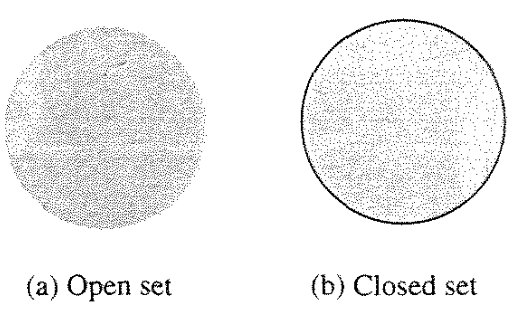
\includegraphics[scale=0.8]{fig2.5}
%  \caption{Illustration d'ensembles ouverts et fermés}
%\end{figure}

\vspace{4mm}
\noindent
\textbf{Exemple 2.1.11} Quelques exemples d'ensembles ouverts et fermés:

\begin{enumerate}
  \item L'ensemble de $(x, y)$ tel que $x^2-2yx = 0$ est fermé dans $\mathbb{R}^2$. (Chaque point est un point frontière.)
  \item L'ensemble de $(x, y)$ tel que $x^2y > 3(x - y)$ est ouvert dans $\mathbb{R}^2$.
  \item L'ensemble $\mathbb{Z}$ est fermé dans $\mathbb{R}$. (Chaque point est isolé de tout autre point; chaque point est un point frontière.)
\end{enumerate}

\noindent
En plus des ensembles simples de points dans $\mathbb{R}^n$, il est intéressant d'examiner les ensembles ouverts et fermés sur des espaces métriques plus complexes.

\vspace{4mm}
\noindent
\textbf{Exemple 2.1.12} Soit $X = C[0, T]$. L'ensemble des fonctions $x \in X$ tel que

\begin{equation*}
  d_\infty(x_0, x) < \epsilon,
\end{equation*}

\noindent
qui est représenté sur la figure 2.3(a), est un ensemble ouvert. C'est le voisinage ouvert des fonctions autour de $x_0(t)$.

\vspace{4mm}
\noindent
\textbf{Définition 2.8} Un point $x \in X$ est dit \textbf{un point de regroupement} dans $X$ si chaque voisinage autour de $x$ contient une infinité de points de $X$.

\vspace{4mm}
\noindent
\textbf{Définition 2.9} Le support d'une fonction $f:A \longrightarrow B$ est la fermeture de l'ensemble des éléments $a \in A$ où $f(a) \neq 0$.

\vspace{2mm}
En concluant cette section de définitions, nous résumons comme suit certaines des propriétés topologiques de base des ensembles.

\begin{enumerate}
  \item L'union de n'importe quel nombre (même un nombre infini) d'ensembles ouverts est ouverte. L'intersection de n'importe quel nombre (même un nombre infini) d'ensembles fermés est fermée.
  \item L'intersection d'un nombre infini d'ensembles ouverts n'a pas besoin d'être ouverte. Pour voir ça, soit $A_k = (0, 1 + 1/k)$. Alors, $A_1 \subset A_2 \subset A_3 \subset \cdots$.
  L'intersection de tous ces intervalles, $B = \cap_{k=1}^{\infty} A_k$ est l'intervalle $(0, 1]$, qui n'est pas un ensemble ouvert.
  \item L'union d'un nombre infini d'ensembles fermés n'a pas besoin d'être fermée.
\end{enumerate}

\subsection{Séquences, séquences de Cauchy et complétude}
\noindent
Les séquences de nombres ou de fonctions apparaissent fréquemment dans la théorie et la pratique du traitement du signal. A titre d'exemple, un algorithme itératif tel qu'un filtre adaptatif produit une séquence de vecteurs (poids de filtre).

% PAGE 79
De nombreuses séquences sont générées comme suit: À partir d'un point initial xo dans un espace métrique X, une séquence est obtenue en mettant à jour le dernier point, en incorporant éventuellement de nouvelles données. La mise à jour d'un algorithme itératif peut être écrite de manière abstraite sous la forme

\begin{equation*}
  x_{n+1} = f(x_n, u_n),
\end{equation*}

\noindent
où $f$ est une fonction de mise à jour et $u_n$ est les données d'entrée à la nième itération. Une itération répétée donne la séquence $x_0, x_1, \ldots$.

Si $x_n$ se rapproche finalement d'une valeur pour $n$ suffisamment grand, nous pouvons dire que la séquence $\{x_n\}$ converge. Ceci est indiqué plus précisément dans la définition suivante.

\vspace{4mm}
\noindent
\textbf{Définition 2.10} Si pour chaque $\delta > 0$, il existe un $n_0$ tel que $d(x_n, x^*) < \delta$ pour chaque $n > n_0$ pour une valeur fixe $x^*$, alors la séquence $\{x_n\}$ est dite converger vers $x^*$. Dans ce cas, nous écrivons

\begin{equation*}
  x_n \longrightarrow x^*.
\end{equation*}

\noindent
On dit dans ce cas que $x^*$ est la \textbf{limite} de $x_n$.

Une autre façon de dire cela est la suivante: La séquence $\{x_n\}$ converge vers $x^*$ si et seulement si tout voisinage autour de $x^*$ contient tous les termes $x_n$ pour $n > n_0$. Pour tout voisinage $N$ autour de $x^*$, il existe un $n_0$ tel que $x_n \in N$ quand $n \geq n_0$.

\vspace{4mm}
\noindent
\textbf{Exemple 2.1.13} La convergence peut être appréciée en considérant des séquences qui ne convergent pas. Les séquences

\begin{equation*}
  a_n = n^2,
\end{equation*}
\begin{equation*}
  b_n = 1 + (-1)^n,
\end{equation*}

\noindent
ne convergent pas: la première suite n'est pas bornée, et la seconde suite oscille entre 0 et 2.

Les faits suivants sur les séquences convergentes sont importants:

\begin{enumerate}
  \item Soit $(X, d)$ un espace métrique. La fermeture d'un ensemble $A \subset X$ est l'ensemble de toutes les limites des séquences convergentes de points de $A$.
  \item Un ensemble $A \subset X$ est fermé si et seulement s'il contient la limite de chaque séquence convergente $\{x_n\}$ dont les points se trouvent dans $A$.
\end{enumerate}

\noindent
\vspace{4mm}
\textbf{Exemple 2.1.14} Considérons la séquence de nombres suivante:

\begin{equation*}
  \{1, 1.41, 1.414, 1.4142, 1.41421, \ldots\}.
\end{equation*}

\noindent
Chaque nombre de cette séquence est un nombre rationnel, un élément de $\mathbb{Q}$. Cette séquence converge vers $\sqrt{2}$, qui est un nombre irrationnel.
Puisque la limite de la suite n'est pas dans l'ensemble $\mathbb{Q}$, nous concluons que $\mathbb{Q}$ n'est pas fermé. Cependant, l'ensemble des nombres réels $\mathbb{R}$ est fermé: toute suite convergente dans $\mathbb{R}$ a sa limite dans $\mathbb{R}$.

\vspace{2mm}
Semblable à une limite est un \textbf{point limite}: si la séquence $x_n$, revient infiniment souvent au voisinage d'un point $x^*$, alors $x^*$ est un point limite. Dans la séquence

\begin{equation*}
  b_n = 1 + (-1)^n,
\end{equation*}

\noindent
les points 0 et 2 sont tous deux des points limites (mais pas des limites) de la séquence. S'il existe des points limites d'une suite, on peut prendre une sous-suite qui converge vers une limite.

Le plus grand point limite d'une séquence $\{x_n\}$ est appelé la limite supérieure, ou \textbf{limsup}. Elle s'écrit souvent sous la forme

\begin{equation*}
  \limsup_{n \longrightarrow \infty} x_n.
\end{equation*}

% PAGE 80
\noindent
Le plus petit point limite d'une séquence est appelé limite inférieure, ou \textbf{liminf}. On l'écrit souvent ainsi

\begin{equation*}
  \liminf_{n \longrightarrow \infty} x_n.
\end{equation*}

\noindent
Évidemment, si $lim sup x_n = lim inf x_n$ alors la suite est convergente.

\vspace{4mm}
\noindent
\textbf{Exemple 2.1.15} Considérons la séquence

\begin{equation*}
  c_n = 1+ \frac{1}{n} + (-1)^n.
\end{equation*}

\noindent
Il y a deux points Ilimit: 2 et 0. La sous-séquence $\{c_0, c_2, c_4, \ldots\}$ a pour limite 2 et la sous-séquence $\{c_1, c_3, c_5, \ldots\}$ a pour limite 0. Pour la séquence $\{c_n\}$,

\begin{equation*}
  \limsup_{n \longrightarrow \infty} c_n = 2,
\end{equation*}
\begin{equation*}
  \liminf_{n \longrightarrow \infty} c_n = 0.
\end{equation*}

\vspace{4mm}
\noindent
\textbf{Définition 2.11} Une séquence $\{x_n\}$ dans $\mathbb{R}$ est \textbf{monotone} si

\begin{equation*}
  x_1 \leq x_2 \leq x_3 \leq \cdots
\end{equation*}
\noindent
ou
\begin{equation*}
  x_1 \geq x_2 \geq x_3 \geq \cdots
\end{equation*}

Pour les suites sur les nombres réels, le fait suivant est clair: toute suite monotone bornée est convergente. Puisque la séquence est limitée, la séquence monotone "manque de place" et doit donc avoir un point limite qui (parce que la séquence est monotone) doit être unique.

\vspace{4mm}
\noindent
\textbf{Définition 2.12} Une suite $\{x_n\}$ dans un espace métrique $(X, d)$ est dite une \textbf{suite de Cauchy} si, pour tout $\epsilon > 0$, il existe un $N > 0$ (qui peut dépendre de $\epsilon$) tel que $d(x_n, x_m) < \epsilon$ pour chaque $m, n > N$.

\vspace{2mm}
On peut montrer (voir les exercices) que si une suite converge, c'est une suite de Cauchy. En revanche, il est possible qu'une suite soit une suite de Cauchy et ne soit pas convergente dans $X$.

\vspace{4mm}
\noindent
\textbf{Exemple 2.1.16} Soit $C[a, b]$ l'ensemble des fonctions continues définies sur l'intervalle $[a, b]$. Soit $X = C[-1, 1]$, et considérons la séquence de fonctions $f_n(t)$ définie par

\begin{equation}
  f_n(t) = \begin{cases} 0 & t < -1/n, \\
    nt/2 + 1/2 & -1/n \leq t \leq 1/n, \\
    1 & t > 1/n.
        \end{cases}
\end{equation}

\noindent
Une fonction typique est présentée dans la figure 2.6. Dans l'espace métrique $(X, d_2)$, où $d_2$ est la métrique définie par

\begin{equation*}
  d_2^2(f, g) = \int_{-1}^{1}(f(t) - g(t))^2 dt,
\end{equation*}

%\begin{figure}[h]
%  \centering
%  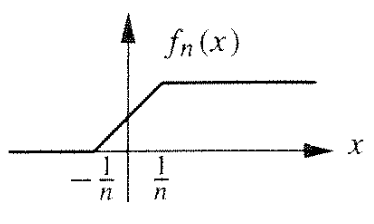
\includegraphics[scale=0.8]{fig2.6}
%  \caption{La fonction $f_n(t)$}
%\end{figure}

% PAGE 81
\noindent
nous trouvons que
\begin{equation*}
  d_2(f_n, f_m) = \frac{1}{6m^3n}(m - n)^2 \quad m > n,
\end{equation*}
\noindent
qui $\longrightarrow 0$ pour $m$ et $n$ grands. Ainsi la séquence est une séquence de Cauchy, mais la fonction limitée
\begin{equation*}
  f(t) = \begin{cases} 0 & t < 0, \\
    1/2 & t = 0, \\
    1 & t > 0.
        \end{cases}
\end{equation*}
\noindent
est une fonction discontinue et n'est donc pas dans $X$. Par conséquent, on ne peut pas dire que $f_n(t)$ est une suite convergente dans $X$.

\vspace{2mm}
L'échec d'une séquence de Cauchy à converger est une déficience - un "trou" - dans l'espace métrique sous-jacent.

\vspace{4mm}
\noindent
\textbf{Définition 2.13} Un espace métrique $(X, d)$ est \textbf{complet} si chaque séquence de Cauchy dans X est convergente dans $X$.

\noindent
Par cette définition, l'espace métrique $(C[a, b], d_2)$ de l'exemple 2.1.16 n'est pas complet: il existe des séquences de Cauchy où la limite n'est pas dans l'espace métrique.

\vspace{4mm}
\noindent
\textbf{Exemple 2.1.17} Le fait qu'un espace métrique soit complet ou non dépend de la métrique utilisée. Considérons l'espace métrique $(C[-1, 1], d_\infty)$, et $d_\infty$ est la métrique

\begin{equation*}
  d_\infty(f, g) = \sup_{t \in [-1, 1]} |f(t) - g(t)|.
\end{equation*}

\noindent
On peut montrer que la séquence $f_n(t)$ n'est pas une séquence de Cauchy dans cet espace métrique, nous ne pouvons donc pas utiliser cette séquence pour tester l'exhaustivité de $(C[a, b], d_\infty)$. Mais on peut encore plaider en faveur de l'exhaustivité de l'espace. 
Soit $x_n(t)$ une suite de Cauchy dans $(C[a, b], d_\infty)$; puis pour tout $\epsilon > 0$,

\begin{equation*}
  \sup_{t \in [-1, 1]} |x_m(t) - x_n(t)| < \epsilon
\end{equation*}

\noindent
pour $m$ et $n$ suffisamment grands, pour que $|x_m(t) - x_n(t)| < \epsilon$ pour chaque $t \in [-1, 1]$. Par conséquent, pour tout $t_0 \in [-1, 1]$ fixe, $x_n(t_0)$ converge vers un certain nombre $x(t_0)$. Collectivement, ceux-ci définissent une fonction $x(t)$. 
Pour être complet, nous devons montrer que $x(t) \in C[a, b]$; en d'autres termes, qu'il est continu. Soit $n$ suffisamment grand pour que $|x_n(t) - x(t)| < \epsilon/3$. Soit $\delta$ déterminé de telle sorte que $|x_n(t) - x_n(t_0)| < \epsilon/3$ quand $|t - t_0| < \delta$. (Puisque $x_n(t)$ est continu, un tel $\delta$ existe.) Alors

\begin{equation*}
  |x(t) - x(t_0)| = |(x(t) - x_n(t)) + (x_n(t) - x_n(t_0)) + (x_n(t_0) - x(t_0))|
\end{equation*}
\begin{equation*}
  \leq |x(t) - x_n(t)| + |x_n(t) - x_n(t_0)| + |x_n(t_0) - x(t_0)| < \epsilon,
\end{equation*}
\noindent
où la première inégalité découle de l'inégalité triangulaire. Ainsi on voit que pour $|t - t_0| < \delta$ on a $|x(t) - x(t_0)| < \epsilon$, donc $x(t)$ doit être continu.
\vspace{2mm}

En examinant la convergence des séquences (comme le résultat d'un algorithme itératif), il est généralement plus facile de montrer qu'une séquence est une séquence de Cauchy que de montrer qu'il s'agit d'une séquence convergente. 
Pour déterminer si une séquence est de Cauchy, il suffit d'examiner la séquence et d'établir que les points deviennent suffisamment proches. En revanche, établir une convergence nécessite des informations autres que la séquence; 
à savoir, la valeur limite de la séquence. Cependant, si l'espace sous-jacent est complet, il suffit alors d'établir qu'une séquence est une séquence de Cauchy pour établir la convergence. Pour cette raison, nous supposerons 
généralement que le travail sur les espaces de fonctions s'effectue dans un espace métrique complet.

\vspace{4mm}
\noindent
\textbf{Exemple 2.1.18} Un exemple d'espace incomplet est l'espace métrique $(\mathbb{Q}, d_1)$, l'ensemble des nombres rationnels. Dans cet espace, la suite $\{1, 1.41, 1.414,$ $1.4142, 1.41421, \ldots\}$, la suite se rapprochant de $\sqrt{2}$, 
est une suite de Cauchy, mais elle n'est pas convergente dans $\mathbb{Q}$, puisque $\sqrt{2}$ n'est pas rationnel.

% PAGE 82
\vspace{7mm}

% Box 2.2 The measure of a set
\fbox{%
    \parbox{\textwidth}{%
\textbf{Encadré 2.2: La mesure d'un ensemble}
\par\noindent\rule{\textwidth}{1pt}

Étant donné un intervalle réel $S = [a, b)$, la mesure de $S$ est simplement la longueur de l'intervalle, $\mu(S) = b - a$. Pour un ensemble qui est l'union d'intervalles disjoints, $S = S_1 \cup S_2 \cup \cdots$, où $S_i \cap S_j = \emptyset$, la mesure est la somme des mesures individuelles,

\begin{equation*}
  \mu(S) = \mu(S_1) + \mu(S_2) + \cdots.
\end{equation*}

Un ensemble de nombres réels est dit avoir une mesure nulle si, pour tout $\epsilon > 0$, l'ensemble peut être couvert par une collection d'intervalles ouverts dont la longueur totale est $< \epsilon$. Un seul polnt a la mesure 0; il en va de même pour une collection finie de points isolés. 
Tout ensemble dénombrable de points a une mesure nulle, car autour du nième point un intervalle ouvert de longueur $\epsilon/2^n$ peut être placé. La longueur totale de l'ensemble dénombrable est donc inférieure ou égale à

\begin{equation*}
  \epsilon \left({\frac{1}{2} + \frac{1}{4} + \frac{1}{8} + \cdots}\right) = \epsilon
\end{equation*}

La mesure des ensembles dans $\mathbb{R}^n$ est définie en trouvant les aires, les volumes, etc. des ensembles dans $\mathbb{R}^n$.
}%
}
\vspace{7mm}

\noindent
En généralisant les résultats de l'exemple 2.1.16, on peut montrer que $(C[a, b], d_p)$ n'est pas un espace métrique complet pour $p < \infty$. Cependant, l'espace $(L_p[a, b], d_p)$ est un espace métrique complet.

\subsection{Détails techniques associés aux espaces* $L_p$ et $L_\infty$}
\noindent
Il existe plusieurs détails techniques associés à l'espace $L_p$, qui méritent au moins une brève considération.

\begin{enumerate}
  \item Considérons les fonctions définies par
  
  \begin{equation*}
    f_1(t) = \begin{cases} sin(t) & 0 \leq t \leq 4, \\
      0 & sinon;
          \end{cases} \quad \quad \quad
    f_2(t) = \begin{cases} sin(t) & 0 \leq t \leq 4, t \neq 2 \\
      5 & t = 2, \\
      0 & sinon.
          \end{cases}
  \end{equation*}
  \noindent
  Ces fonctions ne sont évidemment pas égales en tout point. Cependant, pour tout $p$ compris dans l'intervalle $1 \leq p < \infty$, $d_p(f_1, f_2) = 0$. Nous avons donc des fonctions qui ne sont pas égales mais pour lesquelles la métrique est nulle, en violation de l'exigence M3 pour les métriques, comme indiqué dans la définition 2.1. 
  Les fonctions $f_1(t)$ et $f_2(t)$ sont dites différentes sur un \textit{ensemble de mesures zéro}, ou être égal \textit{presque partout}, abrégé en p.p. (Voir encadré 2.2.)

  Pour nos besoins, les fonctions $f$ et $g$ pour lesquelles $d_p(f, g) = 0$ sont dites égales, même si elles ne sont pas égales en tout point. Ainsi, lorsque nous parlons d'une fonction, nous faisons en réalité référence à toute une classe de fonctions qui diffèrent sur un ensemble de mesures zéro. 
  Donc "égalité" ne signifie pas nécessairement égalité en tout point !
  \vspace{4mm}

  \noindent
  \textbf{Exemple 2.1.19} Il ressort de la théorie des signaux élémentaires qu'une fonction périodique peut être représentée à l'aide d'une série de Fourier. La fonction d'onde carrée périodique définie par

  \begin{equation*}
    f(t) = \begin{cases} 0 & - \frac{1}{2} \leq t < - \frac{1}{4}, \\
      1 &  - \frac{1}{4} \leq t \leq - \frac{1}{4}, \\
      0 & \frac{1}{4} < t < \frac{1}{2},
          \end{cases}
  \end{equation*}

  % PAGE 83

  %\begin{figure}[h]
  %  \centering
  %  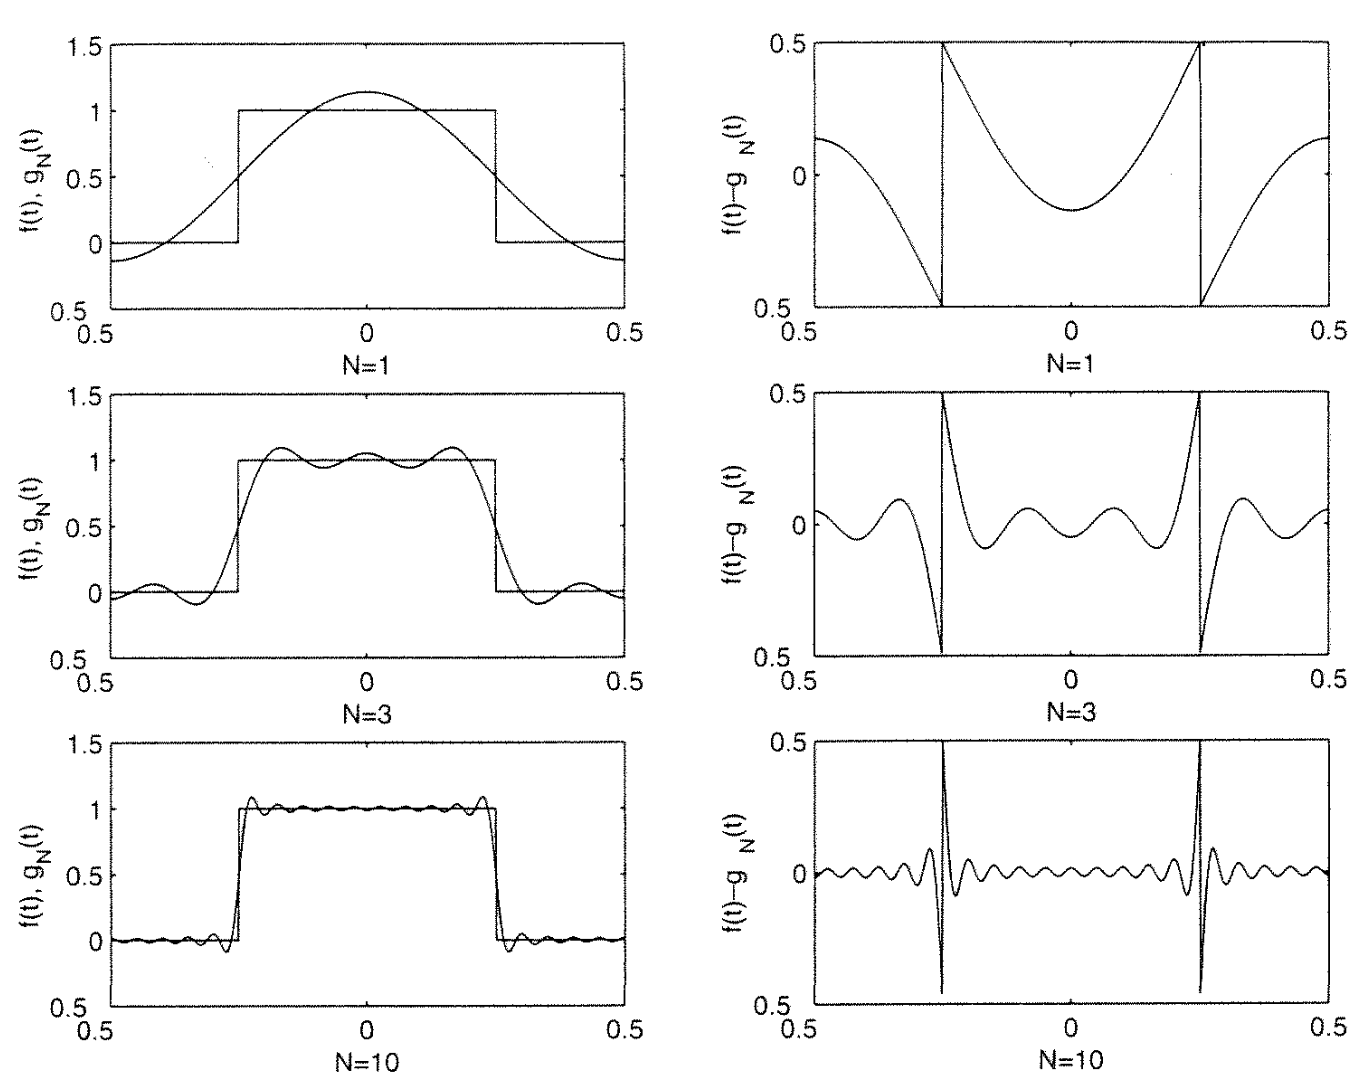
\includegraphics[scale=0.8]{fig2.7}
  %  \caption{Illustration du phénomène Gibbs}
  %\end{figure}

  \noindent
  a la série de Fourier

  \begin{equation}
    f(t) = \frac{1}{2} + \frac{1}{\pi}  \left[2cos2\pi t - \frac{2}{3}cos6\pi t + \frac{2}{5}cos10\pi t + \cdots \right] = g(t).
  \end{equation}

  \noindent
  Alors, par convergence de la série de Fourier on a

  \begin{equation*}
    d_2(f(t), g(t)) = \left[ \int_{-1/2}^{1/2} (f(t) - g(t))^2dt \right]^{1/2} = 0.
  \end{equation*}

  \noindent
  Cependant, on sait également que pour les fonctions discontinues, le phénomène de Gibbs se produit: à un point de discontinuité, il y a un dépassement supérieur ou inférieur, quel que soit le nombre de termes pris dans la sommation. 
  La figure 2.7 illustre la nature de la convergence en montrant la somme dans (2.7) tronquée à $N$ termes, pour $N = 1, 3$ et $10$ termes dans la sommation, les tracés de gauche montrant la fonction et son $N$-terme de Fourier représentation $g_N(t)$, 
  et les tracés de droite montrant l'erreur $f(t) - g_N(t)$. L'erreur point par point converge vers zéro partout sauf aux points de discontinuité, où elle \textit{ne converge jamais vers zéro}. 
  Cependant, comme la largeur de l'emplacement de l'erreur devient de plus en plus étroite, l'intégrale du carré de l'erreur se rapproche de 0 lorsque $N \longrightarrow \infty$.

  \item L'espace $(L_p[a, b], d_p)$ est plus grand que l'espace $(C[a, b], d_p)$, dans le sens où le premier contient le second. Cela est vrai car il y a des fonctions dans $L_p$, qui ne sont pas continues, alors que toutes les fonctions dans $C[a, b]$ sont aussi des fonctions dans $L_p$ (pourquoi ?). 
  $L_p$ est un "achèvement" de $C[a, b]$: les séquences dans $C[a, b]$ qui n'ont pas de limite dans $C[a, b]$ ont une limite dans $L_p$.

  \item En fait, $L_p$ est un espace de fonctions suffisamment grand pour que le concept d'intégration que nous apprenons dans le calcul de base, l'intégrale de Riemann, ne s'applique pas systématiquement à toutes les fonctions de $L_p$. Rappelons que l'intégrale de Riemann est définie comme la limite d'une somme 
  $\sum f(x_i) \Delta x_i$ où les $x_i$, sont choisis comme points à l'intérieur de $\Delta x_i$. Il existe des fonctions dans $L_p$ qui ne peuvent pas être intégrées par ce processus limitant.

  % PAGE 84
  \vspace{4mm}
  \noindent
  \textbf{Exemple 2.1.20} L'exemple pathologique habituel d'une telle fonction non intégrable est la fonction définie sur l'intervalle $[0, 1]$ par

  \begin{equation}
    f(t) = \begin{cases} 1 & si \ t \ est \ rationnel, \\
      0 &  si \ t \ est \ irrationnel.
          \end{cases}
  \end{equation}

  \noindent
  Dans l'intégrale de Riemann, si les points $x_i$ sont choisis comme rationnels, alors $\int_{0}^{1}f(t)dt = 1$. Si les points $x_i$ sont choisis comme irrationnels, alors $\int_{0}^{1}f(t)dt = 0$. Par sélection minutieuse des points $x_i$, l'intégrale peut prendre \textit{n'importe} quelle valeur comprise entre 0 et 1.
  \vspace{4mm}

  \noindent
  L'intégrale appropriée pour une utilisation dans les espaces $L_p$ est \textit{l'intégrale de Lebesgue}. Pour nos besoins, nous n'aurons pas besoin de nous soucier (au-delà de cette brève mention) des distinctions. Soit $\int_{R}$ l'intégration de Riemann et $\int_{L}$ l'intégration de Lebesgue, les règles suivantes s'appliquent:

  \begin{enumerate}
    \item Si $\int_{R}f(t)dt$ existe, alors $\int_{L}f(t)dt$ existe et $\int_{R}f(t)dt = \int_{L}f(t)dt$
    \item L'intégrale de Lebesgue est linéaire: Pour un scalaire $\alpha$,
    
    \begin{equation*}
      \int_L \alpha f = \alpha \int_L f  \quad \quad \quad  \int_L (f + g) = \int_L f + \int_L g .
    \end{equation*}

    \item Si $\int_L |f(t)|^2 dt$ et $\int_L |g(t)|^2 dt$ existe (sont finis), alors $\int_L f(t)g(t)dt$ et $\int_L (f+g)^2 dt$ le sont aussi.
    \item Si f et g sont égaux sauf sur un ensemble de mesure nulle, alors
    
    \begin{equation*}
      \int_L (f - g) = 0  \quad \quad \quad  \int_L (f - g)^2 = 0.
    \end{equation*}

    \noindent
    Cette dernière règle suffit à couvrir bon nombre de fonctions pathologiques pour lesquelles l'intégrale de Riemann n'a aucune valeur. Par exemple, la fonction $f(t)$ définie dans (2.8) est égale à la fonction $g(t) = 0$, sauf sur un ensemble de mesure nulle (puisque les nombres rationnels forment un ensemble dénombrable). 
    Ainsi, en utilisant l'intégrale de Lebesgue il n'y a pas d'ambiguïté et $\int_{0}^{1}f(t)dt = 0$.
  \end{enumerate}

  \item Lorsqu'il s'agit de la norme $L_\infty$, un autre problème se pose. Considérez la fonction
  
  \begin{equation}
    x(t) = \begin{cases} 1 & t = 0, \\
      0 &  t \neq 0.
          \end{cases}
  \end{equation}

  \noindent
  Pour cette fonction $sup x(t) = 1$. Cependant, $x(t)$ ne diffère de la fonction tout zéro que sur un ensemble de mesure zéro. Comme dans le cas des normes $L_p$ il convient de définir la norme $L_\infty$ de telle sorte que les fonctions égales presque partout aient la même norme. 
  On définit donc la norme $L_\infty$ en trouvant la fonction $y(t)$ qui est égale à $x(t)$ presque partout et qui a le plus petit supremum,

  \begin{equation*}
    ||x||_{\infty} = \inf_{y(t)=x(t) p.p} sup |y(t)|.
  \end{equation*}

  \noindent
  Pour la fonction $x(t)$ dans (2.9), nous trouvons que $y(t) = 0$ satisfait ceci; donc,

  \begin{equation*}
    ||x||_{\infty} = 0.
  \end{equation*}

  \noindent
  La quantité $inf_{y(t)=x(t)} sup |y(t)|$ est appelée le \textit{suprême essentiel} de $x(t)$.
\end{enumerate}

% PAGE 85
\subsection{Espaces vectoriels}

\noindent
Un vecteur de dimension finie x peut s'écrire

\begin{equation*}
  X = \begin{bmatrix}
    x_1 \\
    x_2 \\
    \vdots \\
    x_n \\
  \end{bmatrix}.
\end{equation*}

\lhead[\thepage]{2.2 Espaces vectoriels}
\rhead[Espaces de signalisation]{\thepage}

\noindent
Les éléments du vecteur sont $x_i,i = 1, 2, \ldots, n$. 
Chacun des éléments du vecteur appartient à un ensemble, tel que l'ensemble des nombres réels $x_i \in \mathbb{R}$, ou l'ensemble des entiers $x_i \in \mathbb{Z}$. 
Cet ensemble de nombres est appelé l'ensemble des scalaires de l'espace vectoriel.

La représentation vectorielle de dimension finie est largement utilisée, en particulier pour les signaux à temps discret, dans lesquels les composantes du signal à temps discret forment des éléments dans un vecteur. 
Cependant, pour représenter et analyser des signaux en temps continu, une compréhension plus globale des concepts vectoriels est utile. 
Il est possible de considérer la fonction $x(t)$ comme un vecteur et d'appliquer à l'analyse de $x(t)$ bon nombre des mêmes outils qui pourraient être appliqués à l'analyse d'un vecteur \textbf{x} plus conventionnel. 
Nous utiliserons donc également le symbole $x$ (ou $x(t)$) pour représenter les vecteurs ainsi que le symbole \textbf{x}, préférant le symbole \textbf{x} pour le cas des vecteurs de dimension finie. 
De plus, lors de l'introduction de nouveaux concepts d'espace vectoriel, les vecteurs sont indiqués en caractères gras pour les distinguer des scalaires. 
Remarque: dans la notation manuscrite (comme sur un tableau noir), la police en gras est généralement désignée dans la communauté du traitement du signal par un trait de soulignement, comme dans $\underline{x}$, ou, par souci de concision, par aucune notation supplémentaire. 
Désigner les vecteurs manuscrits avec une flèche en exposant $\overrightarrow{x}$ est plus courant dans la communauté des physiciens.

\vspace{4mm}
\noindent
\textbf{Définition 2.14} Un \textbf{espace vectoriel linéaire} $S$ sur un ensemble de scalaires $R$ est une collection d'objets appelés vecteurs, ainsi qu'une opération additive $+$ et une opération de multiplication scalaire $\cdot$, qui satisfont aux propriétés suivantes:

\begin{enumerate}
  \item[VS1] $S$ forme un groupe par addition. Autrement dit, les propriétés suivantes sont satisfaites.
  
  \begin{enumerate}
    \item Pour tout $x$ et $y \in S$ , $x + y \in S$. (L'opération d'addition est fermée.)$^1$
    \item Il existe un élément d'identité dans $S$, que nous noterons \textbf{0}, tel que pour n'importe quel $x \in S$,
    
    \begin{equation*}
      x + 0 = 0 + x = x.
    \end{equation*}

    \item Pour chaque élément $x \in S$ il existe un autre élément $y \in S$ tel que
    
    \begin{equation*}
      x + y = 0.
    \end{equation*}

    \noindent
    L'élément $y$ est l'inverse additif de $x$ et est généralement noté $-x$.
    \item L'opération d'addition est associative; pour tout $x, y$ et $z \in S$,
    
    \begin{equation*}
      (x + y) + z = x + (y + z).
    \end{equation*}
  \end{enumerate}

  \item[VS2] Pour tout $a, b \in R$ et tout $x$ et $y$ dans $S$,
  
  \begin{align*}
    ax &\in S, \\
    a(bx) &= (ab)x, \\
    (a+b)x &= ax + bx, \\
    a(x+y) &= ax + ay.
  \end{align*}

  % PAGE 86
  \item[VS3] Il existe un élément d'identité multiplicatif $1 \in R$ tel que $1x = x$. Il existe un élément $0 \in R$ tel que $0x = 0$.
  \vspace{4mm}
\end{enumerate}

\noindent
L'ensemble $R$ est l'ensemble des scalaires de l'espace vectoriel.
\vspace{3mm}

L'ensemble des scalaires est le plus souvent considéré comme l'ensemble des nombres réels ou des nombres complexes. Cependant, dans certaines applications, d'autres ensembles de scalaires sont utilisés, tels que des polynômes ou des nombres modulo 256. 
La seule exigence concernant l'ensemble de scalaires est que les opérations d'addition et de multiplication puissent être utilisées comme d'habitude (bien qu'aucun inverse multiplicatif ne soit nécessaire), et qu'il existe un nombre 1 qui est une identité multiplicative. 
Dans ce chapitre, lorsque nous parlons de problèmes tels que les sous-espaces fermés, les sous-espaces complets, etc., on suppose que l'ensemble des scalaires est soit les nombres réels $\mathbb{R}$, soit les nombres complexes $\mathbb{Z}$, puisque ceux-ci sont complets.

Nous parlerons indifféremment d'\textit{espace vectoriel linéaire} ou \textit{d'espace vectoriel}.

\vspace{4mm}
\noindent
\textbf{Exemple 2.2.1} L'espace vectoriel le plus connu est $\mathbb{R}^n$, l'ensemble des n-uplets. Par exemple, si $x_1, x_2 \in \mathbb{R}^4$, et

\begin{equation*}
  x_1 = \begin{bmatrix}
    1 \\
    5 \\
    4 \\
    2 \\
  \end{bmatrix}
  \quad \quad \quad
  x_2 = \begin{bmatrix}
    5 \\
    2 \\
    0 \\
    -2 \\
  \end{bmatrix},
\end{equation*}

alors

\begin{equation*}
  x_1 + x_2 = \begin{bmatrix}
    6 \\
    7 \\
    4 \\
    0 \\
  \end{bmatrix}
  \quad \quad \quad
  3x_1 + 2x_2 = \begin{bmatrix}
    13 \\
    19 \\
    12 \\
    2 \\
  \end{bmatrix}.
\end{equation*}

\noindent
Il existe plusieurs autres espaces vectoriels de dimension finie, dont nous mentionnons quelques-uns.
\vspace{4mm}

\noindent
\textbf{Exemple 2.2.2}

\begin{enumerate}
  \item L'ensemble des matrices $m \times n$ avec des éléments réels.
  \item L'ensemble des polynômes de degré jusqu'à $n$ avec des coefficients réels.
  \item L'ensemble des polynômes à coefficients réels, avec l'addition et la multiplication habituelles modulo le polynôme $p(t) = 1 + t^8$, forme un espace vectoriel linéaire. 
  Nous désignons cet espace vectoriel par $\mathbb{R}[t]/ \langle t^8 + 1 \rangle$.
\end{enumerate}
\vspace{4mm}

\noindent
En plus de ces exemples (dont il sera montré ultérieurement qu'ils ont une dimension finie), il existe de nombreux espaces vectoriels importants qui sont de dimension infinie (d'une manière qui sera précisée dans ce qui suit).

\vspace{4mm}
\noindent
\textbf{Exemple 2.2.3}

\begin{enumerate}
  \item Espaces de séquence: L'ensemble de toutes les séquences infiniment longues $\{x_n\}$ forme un espace vectoriel de dimension infinie
  \item Fonctions continues: L'ensemble des fonctions continues définies sur l'intervalle $[a, b]$ forme un espace vectoriel. Nous désignons cet espace vectoriel par $C[a, b]$.
  \item $L_p[a, b]$: Les fonctions dans $L_p$ forment les éléments d'un espace vectoriel de dimension infinie.
\end{enumerate}

\vspace{4mm}
\noindent
\textbf{Définition 2.15} Soit $S$ un espace vectoriel. Si $V \subset S$ est un sous-ensemble tel que $V$ est lui-même un espace vectoriel, alors $V$ est dit un \textbf{sous-espace} de $S$.

\end{document}